\documentclass[tikz,border=10pt]{standalone}
% Scale s = 0.016162 cm/px, y flipped (y_t = (349 - y_px) * s)
\begin{document}
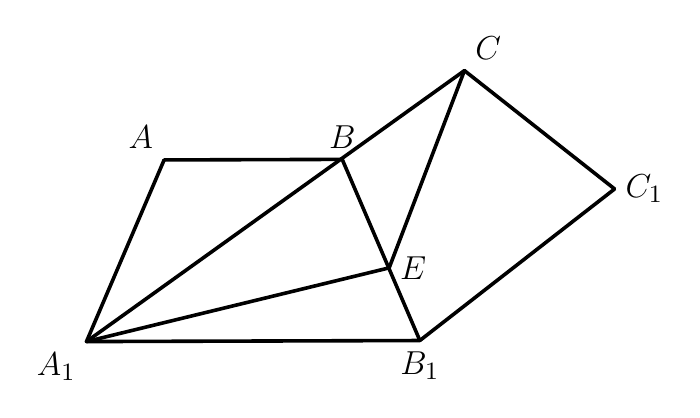
\begin{tikzpicture}[line width=1.3pt, line join=round, line cap=round]
  % Named coordinates
  \coordinate (A1) at (1.2609941047488715,1.1328873354338795);   % (78,279)
  \coordinate (A) at (2.247011034878723,3.4394672509079065);   % (139,136)
  \coordinate (B) at (4.508988965121278,3.4465327490920936);   % (279,136)
  \coordinate (C) at (6.061,4.574);   % (375,66)
  \coordinate (E) at (5.105,2.069);   % (316,221)
  \coordinate (B1) at (5.495005895251129,1.1461126645661204);   % (340,278)
  \coordinate (C1) at (7.968,3.071);   % (493,159)

  % Segments
  \draw (A1) -- (A);          % A1-A
  \draw (A) -- (B);           % A-B horizontal
  \draw (A1) -- (C);          % A1-B-C line (B lies on it)
  \draw (A1) -- (B1);         % bottom base A1-B1, ends exactly at B1
  \draw (A1) -- (E);          % A1-E
  \draw (B) -- (B1);          % B-E-B1 (E lies on it)
  \draw (C) -- (E);           % C-E
  \draw (C) -- (C1);          % C-C1
  \draw (C1) -- (B1);         % C1-B1

  % Labels
  \node[above left] at (A) {\fontsize{13}{15.6}\selectfont $A$};
  \node[above] at (B) {\fontsize{13}{15.6}\selectfont $B$};
  \node[above right] at (C) {\fontsize{13}{15.6}\selectfont $C$};
  \node[right] at (E) {\fontsize{13}{15.6}\selectfont $E$};
  \node[below left] at (A1) {\fontsize{13}{15.6}\selectfont $A_1$};
  \node[below] at (B1) {\fontsize{13}{15.6}\selectfont $B_1$};
  \node[right] at (C1) {\fontsize{13}{15.6}\selectfont $C_1$};
\end{tikzpicture}
\end{document}